\documentclass{article}
\usepackage[utf8]{inputenc}

\title{Mengenal Kecerdasan Buatan dan Scikit-Learn}
\author{Mauliddhia Restu Shafina\\D4 Teknik Informatika 3C\\1.18.4.101}




\usepackage{natbib}
\usepackage{graphicx}

\begin{document}

\maketitle

\section{Teori}

\subsection{Definisi, Sejarah, dan perkembangan Kecerdasan Buatan}
Kecerdasan Buatan merupakan simulasi dari kecerdasan yang dimiliki oleh manusia. Kecerdasan buatan ini, diimplementasikan dengan mesin dan di program agar memiliki kemampuan untuk menampilkan perilaku yang dianggap sama cerdasnya dengan manusia. Kecerdasan buatan yang merupakan bidang ilmu komputer ini telah berkembang sangat pesat di 20 tahun terakhir seiring dengan kebutuhan perangkat cerdas pada rumah tangga dan industry.\\

\textit{Artificial Intelligence} atau Kecerdasan Buatan mulai muncul sekitar tahun 1940 dan 1950 sejak adanya komputer. Munculnya \textit{Artificial Intelligence} ini memberikan banyak keuntungan seperti memiliki sifat permanen, artinya bisa digunakan secara berulang-ulang dimana saja dan kapan saja. Kecerdasan Buatan ini juga menawarkan kemudahan yang mana data yang telah disimpan sebelumnya akan mudah untuk di akses kembali. \\

Ditahun 1960 - 1970, mulailah berbagai diskusi tentang bagaimana komputer dapat menirukan dengan sedetail mungkin kemampuan otak manusia, saat itu dikategorikan dengan \textit{"classical AI"}. Kemudian pada tahun 1980, saat itu komputer sudah mudah didapatkan dengan harga yang terjangkau yang memudahkan berbagai riset dibidang kecerdasan buatan berkembangan dengan pesat diu berbagai universitas dunia. \\

\subsection{Definisi \textit{Supervised Learning}, Klasifikasi, Regresi, \textit{Unsupervised Learning}, \textit{Data set}, \textit{Training set} dan \textit{Testing set}}

\begin{enumerate}

    \item Pengertian \textit{Supervised Learning}\\
    Merupakan sistem dimana sebuah input dan output data yang kita inginkan sudah tersedia. Input dan output data ini diberi label untuk klasifikasi dasar pembelajaran untuk pemrosesan data yang akan datang. \textit{Supervised learing} ini menyediakan algoritma untuk pembelajaran dengan jumlah diketahui untuk mendukung sebuah penilaian yang akan datang seperti: Regrasi Linear Berganda, Analisis Deret Waktu, \textit{Decision tree}, \textit{Random Forest}, dan \textit{Artificial Neural Network}.
    
    \item Pengertian \textit{Unsupervised Learning}\\
    \textit{Unsupervised Learning} berbeda dengan \textit{Supervised Learning}. \textit{Unsupervised Learning} tidak memiliki data latih, sehingga dari data yang telah ada kita kelompokkan menjadi dua atau tiga bagian begitupun seterusnya. \textit{Unsupervised Learning} ini merupakan pelatihan algoritma kecerdasan buatan menggunakan informasi yang tidak diklasifikasikan atau diberi label dan memungkinkan algoritma untuk bertindak atas informasi tersebut tanpa panduan. Tujuan dari algoritma tersebut adalah untuk mengelompokkan sebuah objek yang hampir mirip atau sama ke dalam area tertentu.
    
    \item Pengertian Regresi\\
    Merupakan bagian dari problem \textit{Supervised Learning}, regrasi ini menggunakan metode statistika.
    
    \item Pengertian Klasifikasi\\
    Merupakan sebuah proses pengelompokan benda berdasarkan ciri-ciri persamaan dan perbedaan. Artinya kita memberitahu mesin tersebut bagaimana cara pengerjaannya berdasarkan kelompok.
    
    \item Pengertian \textit{Data Set}\\
    Merupaskan sebuah setobjek yang merepresentasikan sebuah data dan relasi yang ada di memory. Struktur data set mirip dengan data yang ada didalam sebuah database.Namun, didalam dataset berisi sebuash koleksi dari data tabel dan data relasi.
    
    \item Pengertian \textit{Training Set}\\
    Merupakan sebuah set yang digunakan oleh algoritma klassifikasi. Contohnya adalahdecision tree, bayesian, neural network \textit{decision tree, bayesian}, dan \textit{neural network}.
    
    \item Pengertian \textit{Testing Set}\\
    Merupakan sebuah set yang digunakan untuk mengukur sejauh mana sebuah \textit{classfier} berhasil melakukan klasifikasi dengan benar. \textit{Testing set} berfungsi sebagai materai persetujuan, tapi tidak dapat kita gunakan sampai akhir. Setelah data di optimalkan, kita dapat melakukan pengujian jaringan saraf terhadap pengambilan sampel acak. Kemudian hasil yang diperolah harus valid bahwa jaringan kita akurat dalam mengenali gambar.
    
\end{enumerate}
 
\section{Instalasi}

\subsection{Instalasi library scikit dari anaconda, mencoba kompilasi dan uji coba ambil contoh kode dan lihat variabel explorer}

\begin{enumerate}

    \item Langkah pertama, pastikan kita sudah menginstall anaconda terelebih dahulu. Lalu, jangan lupa untuk download \textit{library scikit-learn}. 
    
    \item Buka cmd pada laptop, ketikkan \begin{verbatim}
        pip install -U scikit-learn \end{verbatim}
    \begin{figure}[!htbp]
            \centering
            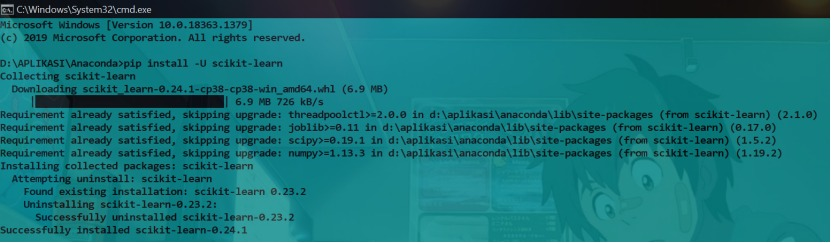
\includegraphics[width=10cm,height=3cm]{figures/1184101/chapter1/1.jpeg}
            \caption{Tampilan installasi \textit{scikit-learn}}
            \label{penanda}
            \end{figure}
    
    \item Melihat versi \textit{scikit-learn} yang telah terinstall pada windows \begin{verbatim}
        python -m pip show scikit-learn \end{verbatim}
    \begin{figure}[!htbp]
            \centering
            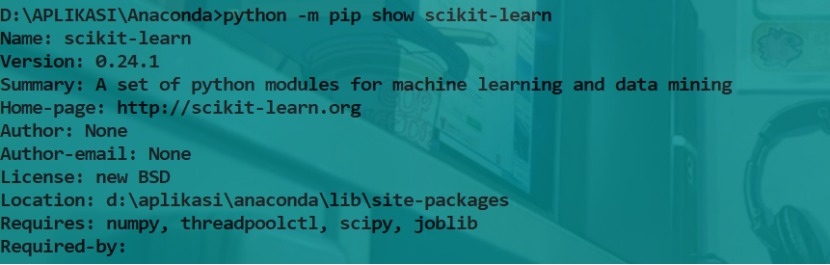
\includegraphics[width=10cm,height=3cm]{figures/1184101/chapter1/2.jpeg}
            \caption{Tampilan installasi \textit{scikit-learn}}
            \label{penanda}
            \end{figure}
    
    \item Melihat isi dalam \textit{scikit-learn} yang sudah terinstall pada windows\begin{verbatim}
        python -m pip show scikit-learn \end{verbatim}
    \begin{figure}[!htbp]
            \centering
            
\includegraphics[width=10cm,height=0.5cm]{figures/1184101/chapter1/3.jpeg}
            \caption{Tampilan installasi \textit{scikit-learn}}
            \label{penanda}
            \end{figure}
    \end{enumerate}
    
\subsection{Mencoba \textit{Loading an example datasets}, menjelaskan maksud dari tulisan tersebut dan mengartikan perbaris}

     \begin{figure}[!htbp]
            \centering
            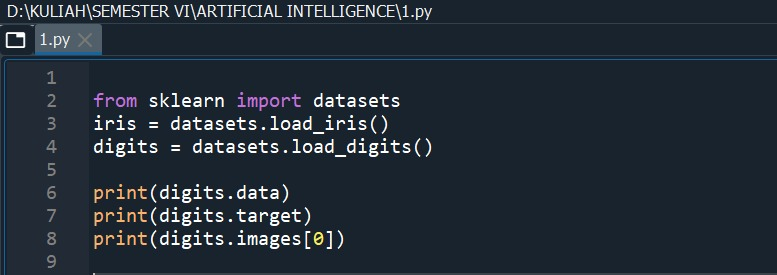
\includegraphics[width=10cm,height=2cm]{figures/1184101/chapter1/4.jpeg}
            \caption{Tampilan perintah \textit{Loading an example datasets}}
            \label{penanda}
            \end{figure}
    
    
        \begin{verbatim}
        from sklearn import datasets \end{verbatim}
        Perintah diatas digunakan untuk memanggil \textit{class} datasets dari library sklearn.
        \begin{verbatim}
        iris = datasets.load_iris()
        digits = datasets.load_digits() \end{verbatim}
        Perintah diatas digunakan untuk memuat \textit{datasets iris} dan \textit{datasets digits} dari package sklearn.
        \begin{verbatim}
        print(digits.data) 
        print(digits.target) 
        print(digits.images[0])
        \end{verbatim}
        Perintah diatas digunakan untuk menampilkan hasil dari variabel data, variabel target, dan variabel images.
    

    \begin{figure}[!htbp]
            \centering
            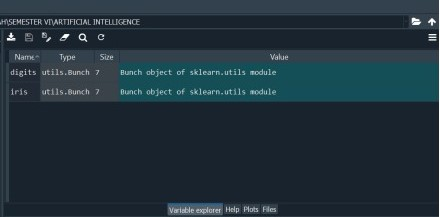
\includegraphics[width=10cm,height=3cm]{figures/1184101/chapter1/18.jpeg}
            \caption{Tampilan variabel explorer pada \textit{Loading an example datasets}}
            \label{penanda}
            \end{figure}
    \begin{figure}[!htbp]
            \centering
            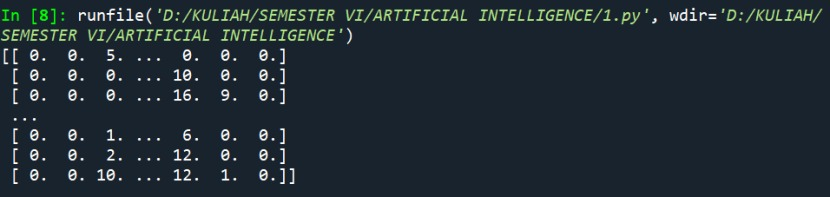
\includegraphics[width=10cm,height=3cm]{figures/1184101/chapter1/6.jpeg}
            \caption{Tampilan perintah \textit{print digits data}}
            \label{penanda}
            \end{figure}
    \begin{figure}[!htbp]
            \centering
            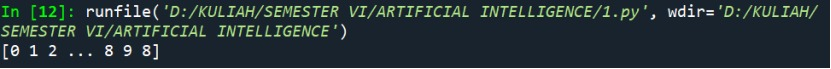
\includegraphics[width=10cm,height=1cm]{figures/1184101/chapter1/7.jpeg}
            \caption{Tampilan perintah \textit{print digits target}}
            \label{penanda}
            \end{figure}
    \begin{figure}[!htbp]
            \centering
            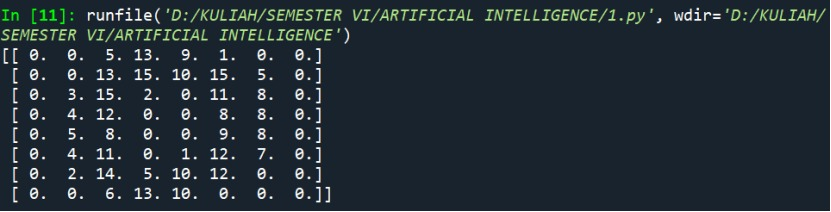
\includegraphics[width=10cm,height=3cm]{figures/1184101/chapter1/8.jpeg}
            \caption{Tampilan perintah \textit{print digits images}}
            \label{penanda}
            \end{figure}
    
\subsection{Mencoba \textit{Learning and Predicting}, menjelaskan maksud dari tulisan tersebut dan mengartikan perbaris}

\begin{figure}[!htbp]
            \centering
            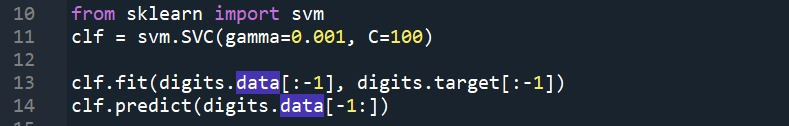
\includegraphics[width=10cm,height=2cm]{figures/1184101/chapter1/9.jpeg}
            \caption{Tampilan perintah \textit{Learning and Predicting}}
            \label{penanda}
            \end{figure}
    
    
        \begin{verbatim}
        from sklearn import svm \end{verbatim}
        Perintah diatas digunakan untuk memanggil \textit{class} svm dari library sklearn.
        \begin{verbatim}
        clf = svm.SVC(gamma=0.001, C=100.) \end{verbatim}
        Perintah diatas digunakan untuk memberikan nilai gamma secara manual.
        \begin{verbatim}
        clf.fit(digits.data[:-1], digits.target[:-1])
       \end{verbatim}
        Perintah diatas csf berfungsi sebagai classifier dan set latihan dengan metode fit.
        \begin{verbatim}
        clf.predict(digits.data[-1:])
        \end{verbatim}
        Perintah diatas digunakan untuk memprediksi nilai baru dari digit data.
    
    \begin{figure}[!htbp]
            \centering
            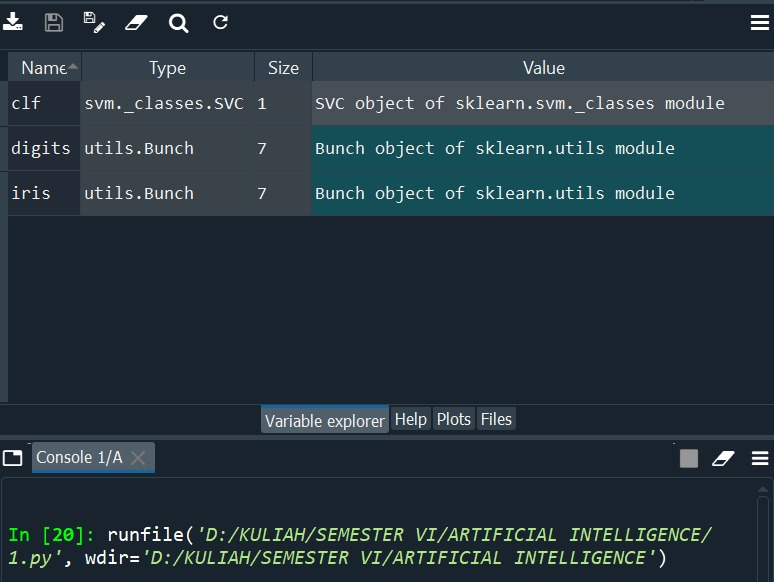
\includegraphics[width=10cm,height=6cm]{figures/1184101/chapter1/10.jpeg}
            \caption{Tampilan variabel explorer pada \textit{Learning and Predicting}}
            \label{penanda}
            \end{figure}

\subsection{Mencoba \textit{Model Persistence}, menjelaskan maksud dari tulisan tersebut dan mengartikan perbaris}

    \begin{figure}[!htbp]
            \centering
            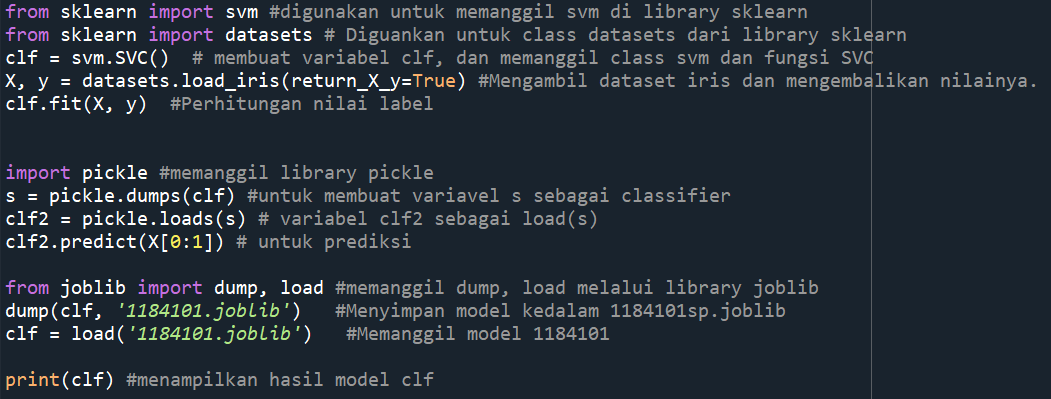
\includegraphics[width=10cm,height=4cm]{figures/1184101/chapter1/19.PNG}
            \caption{Tampilan \textit{Model Persistence}}
            \label{penanda}
            \end{figure}

\begin{verbatim}
    from sklearn import svm
    from sklearn import datasets
\end{verbatim}
Perintah diatas sama-sama digunakan untuk memanggil class svm dan datasets pada library sklearn.

\begin{verbatim}
    clf = svm.SVC()
\end{verbatim}
Perintah diatas digunakan untuk membuat variabel clf dan memanggil class svm dan fungsi SVC.

\begin{verbatim}
    X, y = datasets.load_iris(return_X_y=True)
\end{verbatim}
Perintah diatas digunakan untuk mengambil dataset iris dan mengembalikan nilainya.

\begin{verbatim}
    clf.fit(X, y)
\end{verbatim}
Perintah diatas digunakan untuk menghitung nilai label.

\begin{verbatim}
    import pickle
\end{verbatim}

\begin{verbatim}
     s = pickle.dumps(clf)
\end{verbatim}
Perintah diatas untuk membuat variavel s sebagai classifier
\begin{verbatim}
    clf2 = pickle.loads(s)
    clf2.predict(X[0:1])
\end{verbatim}
Perintah diatas diigunakan untuk variabel clf2 sebagai load(s) dan untuk prediksi x.

\begin{verbatim}
    from joblib import dump, load    
\end{verbatim}
Perintah diatas digunakan untuk memanggil dump, load melalui library joblib.

\begin{verbatim}
    dump(clf, '1184101.joblib')
    clf = load('1184101.joblib')
\end{verbatim}
Perintah diatas digunakan untuk menyimpan model kedalam 1184101sp.joblib dan untukk memanggil model 1184101.

\begin{verbatim}
    print(clf)    
\end{verbatim}
Perintah diatas digunakan untuk menampilkan hasil model clf.

    \begin{figure}[!htbp]
            \centering
            
\includegraphics[width=5cm,height=5cm]{figures/1184101/chapter1/20.PNG}
            \caption{Tampilan apabila telah membuat \textit{Model Persistence}}
            \label{penanda}
            \end{figure}

\subsection{Mencoba \textit{Convention}, menjelaskan maksud dari tulisan tersebut dan mengartikan perbaris}

    \begin{figure}[!htbp]
            \centering
            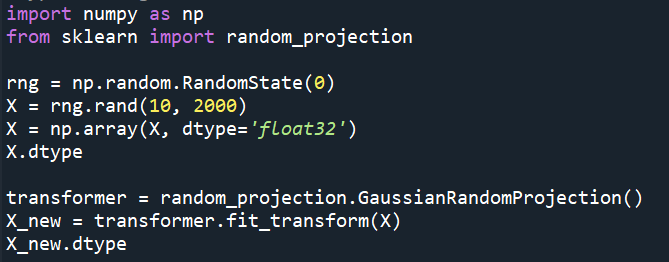
\includegraphics[width=10cm,height=4cm]{figures/1184101/chapter1/21.PNG}
            \caption{Tampilan \textit{convention}}
            \label{penanda}
            \end{figure}

    \begin{figure}[!htbp]
            \centering
            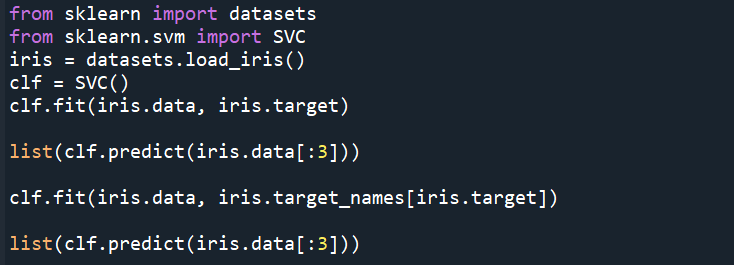
\includegraphics[width=10cm,height=4cm]{figures/1184101/chapter1/22.PNG}
            \caption{Tampilan \textit{convention}}
            \label{penanda}
            \end{figure}
            
    \begin{figure}[!htbp]
            \centering
            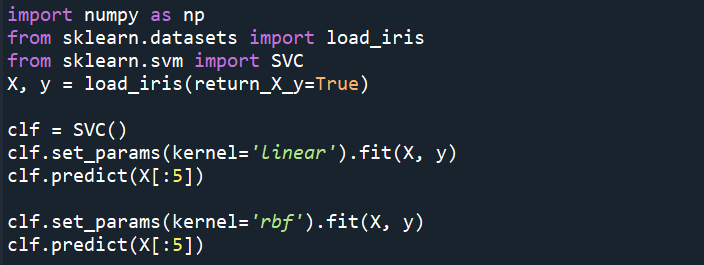
\includegraphics[width=10cm,height=4cm]{figures/1184101/chapter1/23.PNG}
            \caption{Tampilan \textit{convention}}
            \label{penanda}
            \end{figure}
            
    \begin{figure}[!htbp]
            \centering
            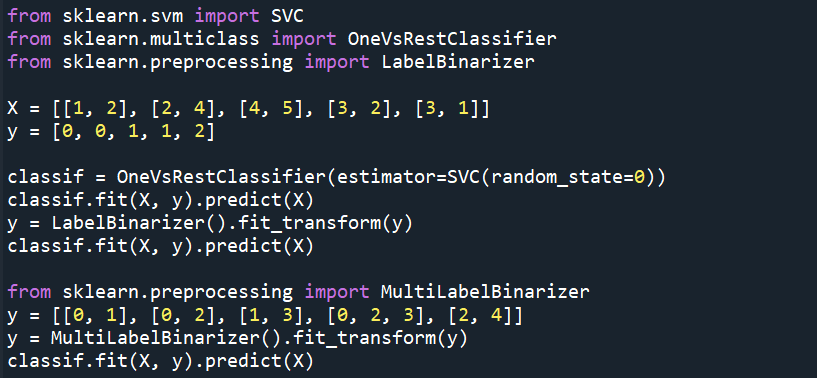
\includegraphics[width=10cm,height=4cm]{figures/1184101/chapter1/24.PNG}
            \caption{Tampilan \textit{convention}}
            \label{penanda}
            \end{figure}

    \begin{figure}[!htbp]
            \centering
            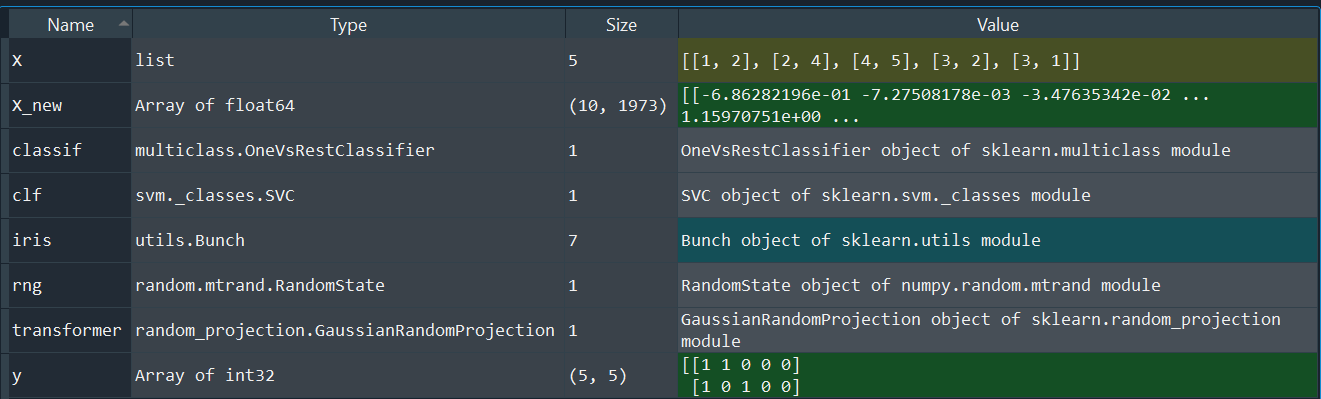
\includegraphics[width=10cm,height=4cm]{figures/1184101/chapter1/25.PNG}
            \caption{Tampilan variabel explorer \textit{convention}}
            \label{penanda}
            \end{figure}
            
\section{Penanganan Eror}
\subsection{\textit{Screenshot} eror}
    
    \begin{figure}[!htbp]
            \centering
            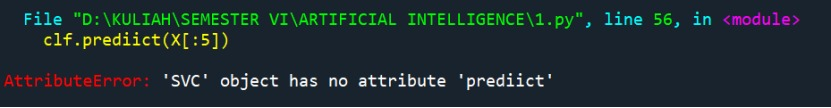
\includegraphics[width=10cm,height=1.5cm]{figures/1184101/chapter1/12.jpeg}
            \caption{Tampilan eror 1}
            \label{penanda}
            \end{figure}
            
    \begin{figure}[!htbp]
            \centering
            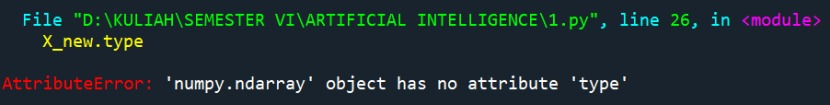
\includegraphics[width=10cm,height=1.5cm]{figures/1184101/chapter1/13.jpeg}
            \caption{Tampilan eror 2}
            \label{penanda}
            \end{figure}
            
    \begin{figure}[!htbp]
            \centering
            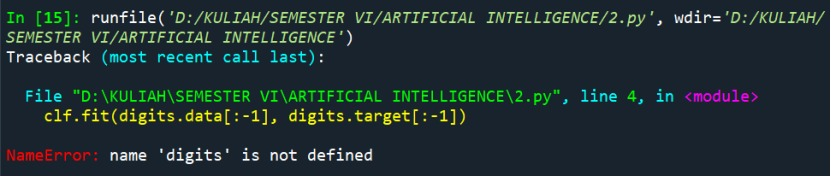
\includegraphics[width=10cm,height=2cm]{figures/1184101/chapter1/15.jpeg}
            \caption{Tampilan eror 3}
            \label{penanda}
            \end{figure}
            
\subsection{Kode eror dan jenis eror}
\begin{enumerate}
    \item Eror 1
\begin{verbatim}
    clf.prediict(X[:5])
\end{verbatim}
Pada eror 1, terjadi kesalahan pada penulisan kata predict.     \item Eror 2
\begin{verbatim}
    X = np.ndarray(X, dtype='float32')
\end{verbatim}
Pada eror 2, terjadi kesalahan pada penulisan kata array.
    \item Eror 3
\begin{verbatim}
    clf.fit(digits.data[:-1], digits.target[:-1])
\end{verbatim}
Pada eror 3, terjadi kesalahan karena penyimpanan pada file yang berbeda.
\end{enumerate}

\subsection{Solusi pemecahan masalah eror}
\begin{enumerate}
    \item Pada eror 1 solusinya harus mengubah penulisan kata prediict menjadi predict.
    \item Pada eror 2 solusinya harus mengubah penulisan kata ndarray menjadi array.
    \item Pada eror 3 solusinya harus menyimpan class digits pada folder yang sama.
\end{enumerate}
\end{document}
